\documentclass[11pt,a4paper]{article}
\usepackage[utf8]{inputenc}
\usepackage[vietnamese]{babel}
\usepackage{amsmath,amssymb}
\usepackage[version=4]{mhchem}
\usepackage{geometry}
\geometry{top=1.5cm,bottom=1.2cm,left=1.4cm,right=1.4cm,headheight=28pt,headsep=12pt,footskip=18pt}
\usepackage{graphicx}
\usepackage{xcolor}
\usepackage{tabularx}
\usepackage{array}
\usepackage{colortbl}
\usepackage{tikz}
\usepackage{fancyhdr}
\usepackage{enumitem}

\graphicspath{{images_quangtrung2_hoa12_2102/}{San_Pham/images_quangtrung2_hoa12_2102/}{C:/Antigravity_Thanh/San_Pham/images_quangtrung2_hoa12_2102/}}

\definecolor{hfRed}{HTML}{D32F2F}
\definecolor{hfGreen}{HTML}{8BC390}
\definecolor{mainGreen}{HTML}{2E7D32}
\definecolor{solBlue}{HTML}{1565C0}
\definecolor{tableGreen}{HTML}{E8F5E9}

\usepackage{ex_test}

\pagestyle{fancy}
\fancyhf{}
\renewcommand{\headrulewidth}{0.75pt}
\renewcommand{\headrule}{\hbox to\headwidth{\color{hfGreen}\leaders\hrule height \headrulewidth\hfill}}
\renewcommand{\footrulewidth}{0.75pt}
\renewcommand{\footrule}{\hbox to\headwidth{\color{hfGreen}\leaders\hrule height \footrulewidth\hfill}}

\fancyhead[L]{\small\itshape\color{hfRed}Tài liệu lưu hành nội bộ}
\fancyhead[R]{\small\color{hfRed}Thầy \textbf{TRẦN VĂN THẠNH} - 0777.470.803}

\fancyfoot[L]{\footnotesize\itshape\color{hfRed}CS1: 6/15 Nguyễn Hoàng, P. Kim Long, TP Huế \quad|\quad CS2: 24 Đặng Thái Thân, TP Huế}
\fancyfoot[R]{\small\textbf{\color{hfRed}Trang \thepage}}

\setlength{\parindent}{0pt}
\setlength{\parskip}{2pt}

\begin{document}


\noindent
\begin{minipage}[t]{0.48\textwidth}
\textbf{SỞ GD \& ĐT GIA LAI}\\
\textbf{TRƯỜNG THPT SỐ 2 QUANG TRUNG}\\
\textbf{ĐỀ CHÍNH THỨC}\\
\textit{(Đề thi có 04 trang)}
\end{minipage}
\hfill
\begin{minipage}[t]{0.48\textwidth}
\raggedleft
\textbf{\color{hfRed}ĐỀ KIỂM TRA GIỮA KỲ I, NĂM HỌC 2026 - 2027}\\
\textbf{MÔN: HÓA HỌC -- KHỐI 12}\\
\textit{Thời gian làm bài: 45 phút (không kể thời gian phát đề)}\\
\textbf{MÃ ĐỀ: 2102}
\end{minipage}

\vspace{4pt}
\noindent
\textit{Họ và tên thí sinh:} \dotfill \textit{Lớp:} \dots\dots\dots \textit{Số báo danh:} \dotfill

\vspace{3pt}
\noindent
\textit{\footnotesize Cho nguyên tử khối của các nguyên tố: C = 12; H = 1; O = 16; Na = 23; Br = 80; N = 14.}

\vspace{2pt}
\hrule height 0.5pt


\vspace{4pt}
\begin{center}
\textbf{\color{hfRed}\large (BẢN GIÁO VIÊN -- CÓ LỜI GIẢI CHI TIẾT)}
\end{center}

\vspace{2pt}
\begin{center}
{\color{hfRed}\textbf{\large BẢNG ĐÁP ÁN RÚT GỌN (DÀNH CHO GIÁO VIÊN - MÃ ĐỀ 2102)}}
\end{center}

\vspace{2pt}
\noindent
\textbf{\color{mainGreen}1. PHẦN I: TRẮC NGHIỆM NHIỀU LỰA CHỌN (16 CÂU - 4,0 ĐIỂM)}
\begin{center}
\renewcommand{\arraystretch}{1.2}
\begin{tabular}{|c|c|c|c|c|c|c|c|c|}
\hline
\rowcolor{tableGreen}
\textbf{Câu} & \textbf{1} & \textbf{2} & \textbf{3} & \textbf{4} & \textbf{5} & \textbf{6} & \textbf{7} & \textbf{8} \\
\hline
\textbf{Đ/A} & \textbf{\color{hfRed}A} & \textbf{\color{hfRed}B} & \textbf{\color{hfRed}A} & \textbf{\color{hfRed}C} & \textbf{\color{hfRed}A} & \textbf{\color{hfRed}C} & \textbf{\color{hfRed}B} & \textbf{\color{hfRed}C} \\
\hline
\rowcolor{tableGreen}
\textbf{Câu} & \textbf{9} & \textbf{10} & \textbf{11} & \textbf{12} & \textbf{13} & \textbf{14} & \textbf{15} & \textbf{16} \\
\hline
\textbf{Đ/A} & \textbf{\color{hfRed}A} & \textbf{\color{hfRed}A} & \textbf{\color{hfRed}D} & \textbf{\color{hfRed}A} & \textbf{\color{hfRed}A} & \textbf{\color{hfRed}D} & \textbf{\color{hfRed}C} & \textbf{\color{hfRed}B} \\
\hline
\end{tabular}
\end{center}

\vspace{2pt}
\noindent
\textbf{\color{mainGreen}2. PHẦN II: TRẮC NGHIỆM ĐÚNG SAI (2 CÂU - 2,0 ĐIỂM)}
\begin{center}
\renewcommand{\arraystretch}{1.2}
\begin{tabular}{|c|c|c|c|c|}
\hline
\rowcolor{tableGreen}
\textbf{Câu hỏi} & \textbf{Lệnh a)} & \textbf{Lệnh b)} & \textbf{Lệnh c)} & \textbf{Lệnh d)} \\
\hline
\textbf{Câu 1} & \textbf{Sai} & \textbf{\color{hfRed}Đúng} & \textbf{Sai} & \textbf{Sai} \\
\hline
\textbf{Câu 2} & \textbf{Sai} & \textbf{\color{hfRed}Đúng} & \textbf{\color{hfRed}Đúng} & \textbf{\color{hfRed}Đúng} \\
\hline
\end{tabular}
\end{center}

\vspace{2pt}
\noindent
\textbf{\color{mainGreen}3. PHẦN III: TRẮC NGHIỆM TRẢ LỜI NGẮN (4 CÂU - 2,0 ĐIỂM)}
\begin{center}
\renewcommand{\arraystretch}{1.2}
\begin{tabular}{|c|c|c|c|c|}
\hline
\rowcolor{tableGreen}
\textbf{Câu hỏi} & \textbf{Câu 1} & \textbf{Câu 2} & \textbf{Câu 3} & \textbf{Câu 4} \\
\hline
\textbf{Đáp án} & \textbf{\color{hfRed}2} & \textbf{\color{hfRed}4} & \textbf{\color{hfRed}3} & \textbf{\color{hfRed}3} \\
\hline
\end{tabular}
\end{center}

\vspace{2pt}
\noindent
\textbf{\color{mainGreen}4. PHẦN IV: TỰ LUẬN (2 CÂU - 2,0 ĐIỂM)}
\begin{itemize}[leftmargin=*,itemsep=1pt]
\item \textbf{Câu 1:} a) Ống 1: phức xanh lam thẫm (nhiều nhóm $\ce{-OH}$ kề nhau). Ống 2: kết tủa đỏ gạch $\ce{Cu2O}$ (nhóm aldehyde $\ce{-CHO}$). b) $\ce{CH2OH[CHOH]4CHO + 2Cu(OH)2 + NaOH -> CH2OH[CHOH]4COONa + Cu2O v + 3H2O}$.
\item \textbf{Câu 2:} a) $\ce{(C17H35COO)3C3H5 + 3NaOH -> 3C17H35COONa + C3H5(OH)3}$. b) $\ce{NaCl}$ bão hòa làm tăng tỉ trọng và giảm độ tan của xà phòng, giúp xà phòng kết tinh nổi lên. c) Khối lượng tristearin tối thiểu: \textbf{\color{hfRed}3,56 kg}.
\end{itemize}

\vspace{4pt}
\hrule color{hfGreen} height 0.5pt


\vspace{6pt}
\noindent
{\color{mainGreen}\textbf{\large PHẦN I. CÂU TRẮC NGHIỆM NHIỀU PHƯƠNG ÁN LỰA CHỌN (4,0 điểm)}}

\textit{Thí sinh trả lời từ câu 1 đến câu 16. Mỗi câu hỏi thí sinh chỉ chọn một phương án.}

\vspace{2pt}


\begin{ex}
Cho các phát biểu sau:
\begin{enumerate}[label=(\arabic*),itemsep=1pt,leftmargin=1.8cm]
\item Alkylamine bậc một tác dụng với nitrous acid ở nhiệt độ thường tạo alcohol và giải phóng khí nitrogen.
\item Dung dịch methylamine tác dụng với dung dịch $\ce{FeCl3}$ tạo kết tủa nâu đỏ $\ce{Fe(OH)3}$.
\item Tripeptide Ala-Gly-Ala tham gia phản ứng màu biuret.
\item Ở điều kiện thường, các amino acid là chất lỏng, ít tan trong nước.
\item Protein trong dung dịch lòng trắng trứng bị đông tụ khi đun nóng.
\item Aniline dễ tham gia phản ứng thế nguyên tử hydrogen ở nhân thơm hơn benzene.
\end{enumerate}
Số phát biểu đúng là
\choice
{\True 5}
{4}
{2}
{3}


\loigiai{
$\bullet$ (1) \textbf{Đúng:} Alkylamine bậc một phản ứng với $\ce{HNO2}$ ở nhiệt độ thường sinh ra alcohol và giải phóng khí $\ce{N2}$ ($\ce{RNH2 + HNO2 -> ROH + N2 ^ + H2O}$).\\
$\bullet$ (2) \textbf{Đúng:} Methylamine có tính base, tạo kết tủa nâu đỏ với $\ce{Fe^3+}$:
\[ \ce{3CH3NH2 + FeCl3 + 3H2O -> Fe(OH)3 v (nâu đỏ) + 3CH3NH3Cl} \]
$\bullet$ (3) \textbf{Đúng:} Tripeptide Ala-Gly-Ala có 2 liên kết peptide nên tham gia phản ứng màu biuret.\\
$\bullet$ (4) \textbf{Sai:} Ở điều kiện thường, các amino acid là chất rắn kết tinh, không màu, tan tốt trong nước.\\
$\bullet$ (5) \textbf{Đúng:} Protein bị đông tụ dưới tác dụng của nhiệt độ cao.\\
$\bullet$ (6) \textbf{Đúng:} Do nhóm $\ce{-NH2}$ đẩy electron làm tăng mật độ electron ở vòng benzene nên aniline dễ phản ứng thế hơn benzene.\\
$\Rightarrow$ Có 5 phát biểu đúng: (1), (2), (3), (5), (6).
}

\end{ex}

\begin{ex}
Mùi tanh của cá chủ yếu do trimethylamine gây ra. Phát biểu nào sau đây \textbf{đúng} về tính chất vật lí của amine?
\choice
{Các amine có số nguyên tử carbon nhỏ đều không tan trong nước}
{\True Trimethylamine là chất khí ở điều kiện thường}
{Tất cả các amine đều là chất rắn ở điều kiện thường}
{Aniline là chất khí, tan tốt trong nước}


\loigiai{
Methylamine, dimethylamine, trimethylamine và ethylamine là những chất khí ở điều kiện thường, tan nhiều trong nước. Aniline là chất lỏng, ít tan trong nước. Phát biểu đúng là B.
}

\end{ex}

\begin{ex}
Dãy nào sau đây gồm polysaccharide?
\choice
{\True Tinh bột, cellulose}
{Saccharose, maltose}
{Glucose, fructose}
{Glucose, saccharose}


\loigiai{
Tinh bột và cellulose là các polysaccharide. Saccharose và maltose là disaccharide. Glucose và fructose là monosaccharide.
}

\end{ex}

\begin{ex}
Saccharose được dùng nhiều trong sản xuất bánh kẹo và nước giải khát. Saccharose có nhiều trong
\choice
{hạt gạo và hạt ngô}
{gỗ và sợi bông}
{\True cây mía, củ cải đường và hoa thốt nốt}
{hạt đang nảy mầm}


\loigiai{
Saccharose có nhiều trong cây mía, củ cải đường và hoa thốt nốt.
}

\end{ex}

\begin{ex}
Amine $\ce{CH3NHCH3}$ có tên gốc - chức là
\choice
{\True dimethylamine}
{methylamine}
{trimethylamine}
{ethylamine}


\loigiai{
$\ce{CH3-NH-CH3}$ có hai nhóm methyl gắn vào nguyên tử N của amine nên có tên gốc - chức là dimethylamine.
}

\end{ex}

\begin{ex}
Ở $\text{pH} = 2$, khi đặt dung dịch glycine trong điện trường thì glycine di chuyển về phía
\choice
{cực dương (+)}
{không di chuyển}
{\True cực âm (--)}
{cả hai cực}


\loigiai{
Ở $\text{pH} = 2$ (môi trường acid mạnh, $\text{pH} < \text{pH}_{\text{I}} \approx 6{,}0$), glycine tồn tại ở dạng cation $\ce{^+H3N-CH2-COOH}$ mang điện tích dương. Do đó trong điện trường, cation di chuyển về phía cực âm (--).
}

\end{ex}

\begin{ex}
Ester $\ce{CH3CH2COOCH3}$ có tên gọi là
\choice
{methyl ethanoate}
{\True methyl propanoate}
{ethyl ethanoate}
{propyl methanoate}


\loigiai{
Gốc alcohol là methyl ($\ce{-CH3}$), gốc acid là propanoate ($\ce{CH3CH2COO-}$) $\Rightarrow$ tên gọi là methyl propanoate.
}

\end{ex}

\begin{ex}
Mỡ lợn, dầu lạc, dầu hướng dương là những nguồn cung cấp chất béo quen thuộc trong bữa ăn hằng ngày. Về cấu tạo, chất béo là
\choice
{ester của glycerol với acid vô cơ}
{monoester của glycerol với acid béo}
{\True triester của glycerol với acid béo}
{diester của glycerol với acid béo}


\loigiai{
Chất béo là triester của glycerol với các acid béo (triglyceride hay triacylglycerol).
}

\end{ex}

\begin{ex}
Dung dịch saccharose không phản ứng với thuốc thử Tollens. Đun nóng dung dịch saccharose với dung dịch $\ce{H2SO4}$ loãng, để nguội rồi trung hòa acid dư bằng dung dịch $\ce{NaOH}$. Thêm thuốc thử Tollens vào dung dịch sau xử lí và đun cách thủy, thấy xuất hiện bạc. Nguyên nhân là do:
\choice
{\True saccharose bị thủy phân tạo thành glucose và fructose, các sản phẩm này phản ứng được với thuốc thử Tollens}
{trong dung dịch, saccharose tồn tại chủ yếu ở dạng mạch hở có nhóm $\ce{-CHO}$}
{acid loãng oxi hóa saccharose thành các chất có nhóm $\ce{-CHO}$}
{acid loãng khử ion $\ce{Ag+}$ trong thuốc thử Tollens thành $\ce{Ag}$}


\loigiai{
Khi đun nóng với acid vô cơ loãng, saccharose bị thủy phân hoàn toàn tạo ra glucose và fructose:
\[ \ce{C12H22O11 + H2O ->[\text{acid},\, t^\circ] C6H12O6 (glucose) + C6H12O6 (fructose)} \]
Cả hai monosaccharide này đều có phản ứng tráng bạc với thuốc thử Tollens.
}

\end{ex}

\begin{ex}
Chất nào sau đây là amine bậc hai?
\choice
{\True $\ce{CH3NHC2H5}$}
{$\ce{(CH3)3N}$}
{$\ce{CH3NH2}$}
{$\ce{C6H5NH2}$}


\loigiai{
$\ce{CH3NHC2H5}$ có nguyên tử N liên kết trực tiếp với 2 gốc hydrocarbon nên là amine bậc hai. $\ce{(CH3)3N}$ là amine bậc ba; $\ce{CH3NH2}$ và $\ce{C6H5NH2}$ là amine bậc một.
}

\end{ex}

\begin{ex}
Ethyl butanoate và ethyl ethanoate là những ester có mùi thơm, được dùng làm chất tạo hương trong công nghiệp thực phẩm và mĩ phẩm. Khi thay thế nhóm $\ce{-OH}$ trong nhóm carboxyl ($\ce{-COOH}$) của carboxylic acid bằng nhóm $-\ce{OR}'$ ($\text{R}'$ là gốc hydrocarbon) thì thu được hợp chất thuộc loại nào sau đây?
\choice
{Amino acid}
{Alcohol}
{Amine}
{\True Ester}


\loigiai{
Theo định nghĩa: Khi thay thế nhóm $\ce{-OH}$ trong nhóm carboxyl của carboxylic acid bằng nhóm $-\ce{OR}'$ thì thu được hợp chất thuộc loại ester.
}

\end{ex}

\begin{ex}
Một cơ sở tận dụng dầu ăn đã qua sử dụng để sản xuất biodiesel. Trong quy trình tái chế, chất béo trong dầu ăn phản ứng với methanol có xúc tác thích hợp, tạo các methyl ester của acid béo và glycerol theo phương trình tổng quát sau:
\[ \ce{(RCOO)3C3H5 + 3CH3OH ->[\text{xúc tác},\, t^\circ] 3RCOOCH3 + C3H5(OH)3} \]
Cơ sở sử dụng $100\text{ kg}$ dầu ăn đã qua sử dụng chứa $88{,}4\%$ triolein theo khối lượng, phần còn lại là tạp chất không tham gia phản ứng và không tạo biodiesel. Cho lượng dầu này phản ứng với methanol dư, hiệu suất chuyển hóa triolein thành methyl oleate đạt $90\%$. Khối lượng biodiesel thu được là bao nhiêu, biết biodiesel trong bài toán chỉ gồm methyl oleate?
\choice
{\True $79{,}92\text{ kg}$}
{$79{,}56\text{ kg}$}
{$88{,}80\text{ kg}$}
{$26{,}64\text{ kg}$}


\loigiai{
$\bullet$ Khối lượng triolein ban đầu: $m_{\text{triolein}} = 100 \times 88{,}4\% = 88{,}4\text{ kg}$.\\
$\bullet$ Phân tử khối triolein $\ce{(C17H33COO)3C3H5}$: $M = 884\text{ g/mol} \Rightarrow n_{\text{triolein}} = \dfrac{88{,}4}{884} = 0{,}1\text{ kmol}$.\\
$\bullet$ Phân tử khối methyl oleate $\ce{C17H33COOCH3}$: $M = 296\text{ g/mol}$.\\
Theo PTHH: $n_{\text{este (LT)}} = 3 \times n_{\text{triolein}} = 0{,}3\text{ kmol} \Rightarrow m_{\text{este (LT)}} = 0{,}3 \times 296 = 88{,}8\text{ kg}$.\\
$\bullet$ Do hiệu suất $H = 90\%$, khối lượng biodiesel thực tế thu được là:
\[ m = 88{,}8 \times 90\% = \mathbf{79{,}92\text{ kg}}. \]
}

\end{ex}

\begin{ex}
Trong sản xuất thực phẩm, dầu thực vật có thể được chế biến thành chất béo có độ rắn cao hơn, dùng làm nguyên liệu sản xuất bơ thực vật. Quá trình hóa học nào sau đây giúp thực hiện sự chuyển đổi này?
\choice
{\True Chất béo lỏng chứa gốc acid béo không no cộng $\ce{H2}$ (có xúc tác, nhiệt độ thích hợp) tạo thành chất béo chứa gốc acid béo no ở dạng rắn}
{Thủy phân chất béo trong dầu thực vật thành glycerol và acid béo}
{Xà phòng hóa chất béo trong dầu thực vật bằng dung dịch $\ce{NaOH}$}
{Oxi hóa chất béo trong dầu thực vật bằng oxygen không khí}


\loigiai{
Quá trình hydrogen hóa (cộng $\ce{H2}$ xúc tác $\ce{Ni}$, đun nóng) chất béo lỏng chứa gốc không no thành chất béo rắn chứa gốc no giúp sản xuất bơ nhân tạo (margarine).
}

\end{ex}

\begin{ex}
Dung dịch glucose $5\%$ được dùng để truyền tĩnh mạch nhằm cung cấp năng lượng nhanh cho bệnh nhân. Glucose thuộc loại carbohydrate nào sau đây?
\choice
{Disaccharide}
{Lipid}
{Polysaccharide}
{\True Monosaccharide}


\loigiai{
Glucose là một monosaccharide.
}

\end{ex}

\begin{ex}
Ethanol sinh học (cồn sinh học) được dùng làm nhiên liệu sinh học, được sản xuất bằng cách lên men các nguyên liệu chứa tinh bột. Từ 1 tấn sắn khô chứa $81\%$ tinh bột về khối lượng, với hiệu suất của toàn bộ quá trình là $70\%$, khối lượng ethanol thu được là
\choice
{$230\text{ kg}$}
{$414\text{ kg}$}
{\True $322\text{ kg}$}
{$460\text{ kg}$}


\loigiai{
Sơ đồ: $\ce{(C6H10O5)_n -> n C6H12O6 -> 2n C2H5OH}$.\\
Cứ $162\text{ kg}$ tinh bột theo lí thuyết sinh ra $2 \times 46 = 92\text{ kg }\ce{C2H5OH}$.\\
Khối lượng tinh bột nguyên chất: $m = 1000 \times 81\% = 810\text{ kg}$.\\
Khối lượng ethanol lí thuyết: $m_{\text{LT}} = \dfrac{810 \times 92}{162} = 460\text{ kg}$.\\
Khối lượng ethanol thực tế thu được với hiệu suất $70\%$:
\[ m_{\text{TT}} = 460 \times 70\% = \mathbf{322\text{ kg}}. \]
}

\end{ex}

\begin{ex}
Tiến hành thí nghiệm như hình vẽ sau: nhỏ một giọt dung dịch methylamine $0{,}1\text{ M}$ lên mẩu giấy quỳ tím đặt trên mặt kính đồng hồ (1), nhỏ một giọt dung dịch aniline $0{,}1\text{ M}$ lên mẩu giấy quỳ tím đặt trên mặt kính đồng hồ (2).
\begin{center}
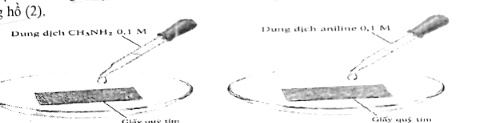
\includegraphics[width=11cm]{images_quangtrung2_hoa12_2102/hinh_cau16_quy_tim.png}
\end{center}
Hiện tượng quan sát được là
\choice
{cả hai mẩu giấy quỳ tím đều chuyển sang màu xanh}
{\True giấy quỳ tím (1) chuyển sang màu xanh, giấy quỳ tím (2) không đổi màu}
{giấy quỳ tím (1) không đổi màu, giấy quỳ tím (2) chuyển sang màu xanh}
{cả hai mẩu giấy quỳ tím đều không đổi màu}


\loigiai{
Methylamine có tính base mạnh hơn ammonia do nhóm alkyl đẩy electron, làm quỳ tím hóa xanh. Aniline có tính base rất yếu do gốc phenyl hút electron mạnh, không làm đổi màu quỳ tím.
}

\end{ex}

\vspace{6pt}
\noindent
{\color{mainGreen}\textbf{\large PHẦN II. CÂU TRẮC NGHIỆM ĐÚNG SAI (2,0 điểm)}}

\textit{Thí sinh trả lời từ câu 1 đến câu 2. Trong mỗi ý a), b), c), d) ở mỗi câu, thí sinh chọn đúng hoặc sai.}

\vspace{2pt}


\begin{ex}
Tinh bột có nhiều trong gạo, ngô, khoai; cellulose là thành phần chính của sợi bông và có trong gỗ. Hai chất này có vai trò quan trọng trong đời sống nhưng khác nhau về cấu tạo và tính chất. Hãy xác định các phát biểu sau là đúng hay sai:
\choiceTF
{Tinh bột và cellulose đều là polysaccharide có công thức tổng quát $\ce{(C6H10O5)_n}$ nên có cấu tạo hoàn toàn giống nhau.}
{\True Trong cơ thể người, tinh bột được thủy phân qua các sản phẩm trung gian, cuối cùng tạo glucose. Glucose được hấp thu vào máu, cung cấp năng lượng hoặc chuyển thành glycogen dự trữ.}
{Tinh bột là chất rắn màu trắng, tan tốt trong nước lạnh.}
{Hồ tinh bột đã trộn với dung dịch iodine mất màu khi đun nóng nhẹ và xuất hiện lại màu xanh tím khi để nguội vì tinh bột đã thủy phân hoàn toàn thành glucose.}


\loigiai{
a) \textbf{Sai.} Tinh bột gồm các gốc $\alpha$-glucose, còn cellulose gồm các gốc $\beta$-glucose, cấu tạo phân tử khác nhau.\\
b) \textbf{Đúng.} Tinh bột bị enzyme amylase thủy phân thành dextrin $\to$ maltose $\to$ glucose. Glucose đi vào máu cung cấp năng lượng hoặc chuyển thành glycogen dự trữ.\\
c) \textbf{Sai.} Tinh bột không tan trong nước lạnh, chỉ trương trong nước nóng tạo hồ tinh bột.\\
d) \textbf{Sai.} Màu biến mất do cấu trúc xoắn của amylose duỗi ra khi đun nóng giải phóng iodine; để nguội cấu trúc xoắn tái lập lại nên màu xanh tím trở lại, không phải do tinh bột bị thủy phân.
}

\end{ex}

\begin{ex}
Một nhóm học sinh tìm hiểu tính chất của protein trong lòng trắng trứng bằng thí nghiệm được mô tả trong hình dưới đây, kết quả thu được dung dịch X.
\begin{center}
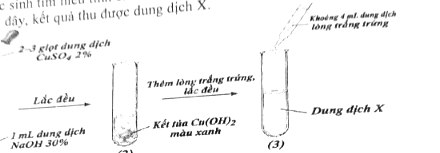
\includegraphics[width=12cm]{images_quangtrung2_hoa12_2102/hinh_p2_cau2_biuret.png}
\end{center}
Hãy xác định các phát biểu sau là đúng hay sai:
\choiceTF
{Nếu thay dung dịch lòng trắng trứng bằng dung dịch glycine thì vẫn xuất hiện màu tím đặc trưng của phản ứng biuret.}
{\True Các protein dạng hình sợi như keratin (trong tóc, móng), collagen (trong da, sụn) không tan trong nước.}
{\True Dung dịch X có màu tím.}
{\True Khi nấu ăn người ta dùng nước ép dứa tươi để làm mềm thịt vì enzyme bromelain trong nước ép dứa tươi có khả năng xúc tác phản ứng thủy phân protein.}


\loigiai{
a) \textbf{Sai.} Glycine là amino acid đơn lẻ, không có liên kết peptide nên không cho phản ứng màu biuret.\\
b) \textbf{Đúng.} Protein dạng sợi (keratin, collagen) không tan trong nước.\\
c) \textbf{Đúng.} Albumin trong lòng trắng trứng tạo phức chất màu tím đặc trưng với $\ce{Cu(OH)2}$ trong môi trường kiềm (phản ứng biuret).\\
d) \textbf{Đúng.} Dứa tươi chứa bromelain là một protease xúc tác thủy phân protein giúp thịt mềm.
}

\end{ex}

\vspace{6pt}
\noindent
{\color{mainGreen}\textbf{\large PHẦN III. CÂU TRẮC NGHIỆM TRẢ LỜI NGẮN (2,0 điểm)}}

\textit{Thí sinh trả lời từ câu 1 đến câu 4. Điền kết quả trả lời vào phiếu làm bài.}

\vspace{2pt}


\begin{ex}
Saccharose được dùng phổ biến làm đường ăn, còn maltose có trong sản phẩm thủy phân tinh bột. Xét các đặc điểm cấu tạo sau:
\begin{enumerate}[label=(\arabic*),itemsep=1pt,leftmargin=1.8cm]
\item Trong cấu tạo phân tử có hai đơn vị monosaccharide liên kết với nhau.
\item Có 8 nhóm $\ce{-OH}$ trong phân tử.
\item Chỉ được tạo thành từ các đơn vị glucose.
\item Có 1 nhóm $\ce{-OH}$ hemiacetal tự do.
\end{enumerate}
Có bao nhiêu đặc điểm đúng với cả saccharose và maltose ở dạng vòng?


\loigiai{
$\bullet$ (1) Đúng: Cả hai đều là disaccharide, gồm 2 đơn vị monosaccharide liên kết qua liên kết glycoside.\\
$\bullet$ (2) Đúng: Đều có CTPT $\ce{C12H22O11}$ với đúng 8 nhóm $\ce{-OH}$ ở dạng mạch vòng.\\
$\bullet$ (3) Sai: Saccharose cấu tạo từ 1 gốc glucose và 1 gốc fructose; chỉ maltose mới từ 2 gốc glucose.\\
$\bullet$ (4) Sai: Saccharose không còn nhóm $\ce{-OH}$ hemiacetal tự do; chỉ maltose còn 1 nhóm.\\
$\Rightarrow$ Có \textbf{2} đặc điểm đúng: (1) và (2).\\
\textbf{Đáp số: 2.}
}

\end{ex}

\begin{ex}
Xà phòng và chất giặt rửa tổng hợp được sử dụng phổ biến trong đời sống. Xét các phát biểu sau về phương pháp sản xuất và cách sử dụng hai loại sản phẩm này:
\begin{enumerate}[label=\alph*),itemsep=1pt,leftmargin=1.5cm]
\item Xà phòng có thể được sản xuất bằng cách đun nóng chất béo với dung dịch $\ce{NaOH}$ hoặc $\ce{KOH}$.
\item Phương pháp chủ yếu để sản xuất chất giặt rửa tổng hợp là đun nóng chất béo với dung dịch kiềm.
\item Trong sản xuất chất giặt rửa tổng hợp, có thể sulfo hoá alkylbenzene rồi trung hoà sản phẩm bằng $\ce{NaOH}$ để thu được sodium alkylbenzenesulfonate.
\item Khi giặt bằng nước cứng, xà phòng tạo kết tủa với ion $\ce{Ca^2+}$, $\ce{Mg^2+}$ nên bị giảm tác dụng giặt rửa.
\item Cần sử dụng xà phòng và chất giặt rửa tổng hợp đúng mục đích, đúng liều lượng theo hướng dẫn, tránh để sản phẩm tiếp xúc với mắt.
\end{enumerate}
Có bao nhiêu phát biểu đúng?


\loigiai{
$\bullet$ a) Đúng: Phản ứng xà phòng hóa chất béo với $\ce{NaOH}/\ce{KOH}$ sinh ra muối của acid béo (xà phòng).\\
$\bullet$ b) Sai: Chất giặt rửa tổng hợp được sản xuất chủ yếu từ dầu mỏ, không phải từ chất béo.\\
$\bullet$ c) Đúng: Sulfo hóa alkylbenzene bằng $\ce{H2SO4}$ đặc rồi trung hòa bằng $\ce{NaOH}$ thu được sodium alkylbenzenesulfonate.\\
$\bullet$ d) Đúng: Trong nước cứng tạo kết tủa calcium/magnesium stearate làm giảm tác dụng tẩy rửa.\\
$\bullet$ e) Đúng: Sử dụng đúng liều lượng và an toàn cho mắt/da tay.\\
$\Rightarrow$ Có \textbf{4} phát biểu đúng: a, c, d, e.\\
\textbf{Đáp số: 4.}
}

\end{ex}

\begin{ex}
Cho $\ce{Cu(OH)2}$ mới tạo vào dung dịch Gly-Ala-Gly trong môi trường kiềm, lắc đều thấy xuất hiện màu tím. Xét các nhận định:
\begin{enumerate}[label=(\arabic*),itemsep=1pt,leftmargin=1.8cm]
\item Gly-Ala-Gly có hai liên kết peptide trong phân tử.
\item Màu tím xuất hiện do peptide tạo phức với ion $\ce{Cu^2+}$ trong môi trường kiềm.
\item Thay Gly-Ala-Gly bằng Gly-Ala vẫn thu được màu tím đặc trưng tương tự.
\item Sau khi thuỷ phân hoàn toàn Gly-Ala-Gly, hỗn hợp sản phẩm không còn cho phản ứng màu biuret.
\end{enumerate}
Có bao nhiêu nhận định đúng?


\loigiai{
$\bullet$ (1) Đúng: Tripeptide có $3 - 1 = 2$ liên kết peptide $\ce{-CO-NH-}$.\\
$\bullet$ (2) Đúng: Các liên kết peptide tạo phức chelate màu tím đặc trưng với ion $\ce{Cu^2+}$ trong kiềm.\\
$\bullet$ (3) Sai: Gly-Ala là dipeptide (chỉ có 1 liên kết peptide), không có phản ứng biuret.\\
$\bullet$ (4) Đúng: Thủy phân hoàn toàn thu được các amino acid tự do (glycine và alanine), không còn liên kết peptide nên không cho phản ứng biuret.\\
$\Rightarrow$ Có \textbf{3} nhận định đúng: (1), (2), (4).\\
\textbf{Đáp số: 3.}
}

\end{ex}

\begin{ex}
Tiến hành thí nghiệm nhỏ aniline loãng vào nước bromine dư như hình sau:
\begin{center}
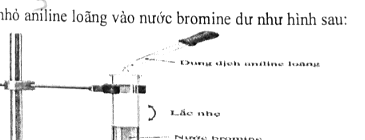
\includegraphics[width=9cm]{images_quangtrung2_hoa12_2102/hinh_p3_cau4_aniline_bromine.png}
\end{center}
Xét các nhận định:
\begin{enumerate}[label=(\arabic*),itemsep=1pt,leftmargin=1.8cm]
\item Xuất hiện kết tủa trắng là 2,4,6-tribromoaniline.
\item Do ảnh hưởng của nhóm $\ce{-NH2}$ lên vòng benzene nên aniline tham gia phản ứng thế nguyên tử hydrogen dễ hơn benzene.
\item Nếu thay dung dịch aniline trong thí nghiệm trên bằng dung dịch alanine thì vẫn thu được kết tủa trắng.
\item Cho $0{,}01\text{ mol}$ aniline phản ứng hoàn toàn với nước bromine dư thì thấy $4{,}8\text{ gam}$ bromine phản ứng.
\end{enumerate}
Có bao nhiêu nhận định đúng?


\loigiai{
$\ce{C6H5NH2 + 3Br2 -> C6H2Br3NH2 v (trắng) + 3HBr}$\\
$\bullet$ (1) Đúng: Kết tủa trắng là 2,4,6-tribromoaniline.\\
$\bullet$ (2) Đúng: Nhóm $\ce{-NH2}$ hoạt hóa vòng thơm làm phản ứng thế halogen xảy ra rất nhanh và dễ dàng.\\
$\bullet$ (3) Sai: Alanine là amino acid no, không phản ứng với nước bromine tạo kết tủa trắng.\\
$\bullet$ (4) Đúng: $n_{\ce{Br2}} = 3 \times n_{\text{aniline}} = 0{,}03\text{ mol} \Rightarrow m_{\ce{Br2}} = 0{,}03 \times 160 = \mathbf{4{,}8\text{ gam}}$.\\
$\Rightarrow$ Có \textbf{3} nhận định đúng: (1), (2), (4).\\
\textbf{Đáp số: 3.}
}

\end{ex}

\vspace{6pt}
\noindent
{\color{mainGreen}\textbf{\large PHẦN IV. TỰ LUẬN (2,0 điểm)}}

\textit{Thí sinh trả lời từ câu 1 đến câu 2. Trình bày chi tiết lời giải vào giấy làm bài thi.}

\vspace{2pt}


\begin{ex}
\textbf{(1,0 điểm)} Để tìm hiểu tính chất hóa học của glucose tiến hành thí nghiệm như sau:
\begin{itemize}[leftmargin=*,itemsep=1pt]
\item \textit{Bước 1:} Cho vào mỗi ống nghiệm (1) và (2) lần lượt $3\text{ mL}$ dung dịch $\ce{NaOH}\ 10\%$, $0{,}6\text{ mL}$ dung dịch $\ce{CuSO4}\ 5\%$ rồi lắc đều. Tiếp tục thêm vào mỗi ống $3\text{ mL}$ dung dịch glucose $5\%$ và lắc đều.
\item \textit{Bước 2:} Giữ ống nghiệm (1) ở nhiệt độ thường, đun nóng nhẹ ống nghiệm (2) bằng đèn cồn trong vài phút. Cách bố trí thí nghiệm được mô tả trong hình.
\end{itemize}
\begin{center}
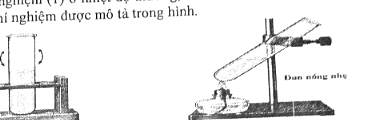
\includegraphics[width=12cm]{images_quangtrung2_hoa12_2102/hinh_p4_cau1_glucose_cuoh2.png}
\end{center}
a) \textit{(0,5 điểm)} Nêu hiện tượng quan sát được ở mỗi ống nghiệm. Mỗi hiện tượng đó chứng tỏ trong phân tử glucose có nhóm chức nào?\\
b) \textit{(0,5 điểm)} Viết phương trình hóa học của phản ứng xảy ra ở ống nghiệm (2).


\loigiai{
a) \textbf{Hiện tượng quan sát được và chứng minh cấu tạo:}
\begin{itemize}[leftmargin=*,itemsep=1pt]
\item \textbf{Ống nghiệm (1) (ở nhiệt độ thường):} Kết tủa xanh lam $\ce{Cu(OH)2}$ bị hòa tan, dung dịch trở nên đồng nhất và có màu xanh lam thẫm (dung dịch phức chất đồng(II) - glucose).\\
$\to$ Chứng minh trong phân tử glucose có \textbf{nhiều nhóm hydroxy ($\ce{-OH}$) kề nhau} (tính chất polyol).
\item \textbf{Ống nghiệm (2) (khi đun nóng nhẹ):} Xuất hiện kết tủa màu đỏ gạch ($\ce{Cu2O}$).\\
$\to$ Chứng minh trong phân tử glucose có \textbf{nhóm aldehyde ($\ce{-CHO}$)} (tính khử trong môi trường kiềm).
\end{itemize}
b) \textbf{Phương trình hóa học xảy ra ở ống nghiệm (2):}
\begin{align*}
\ce{CuSO4 + 2NaOH &-> Cu(OH)2 v + Na2SO4} \\
\ce{2C6H12O6 + Cu(OH)2 &-> (C6H11O6)2Cu + 2H2O} \\
\ce{CH2OH[CHOH]4CHO + 2Cu(OH)2 + NaOH &->[t^\circ] CH2OH[CHOH]4COONa + Cu2O v (đỏ gạch) + 3H2O}
\end{align*}
\textit{(hoặc viết dạng phân tử: $\ce{C6H12O6 + 2Cu(OH)2 + NaOH ->[t^\circ] C6H11O7Na + Cu2O v + 3H2O}$)}
}

\end{ex}

\begin{ex}
\textbf{(1,0 điểm)} Trong phòng thí nghiệm, một nhóm học sinh tiến hành thí nghiệm cho tristearin tác dụng với dung dịch $\ce{NaOH}$ và xử lí sản phẩm theo quy trình minh họa dưới đây để tạo xà phòng (sản phẩm mang tính thực nghiệm và chưa được đánh giá chất lượng sử dụng):
\begin{center}
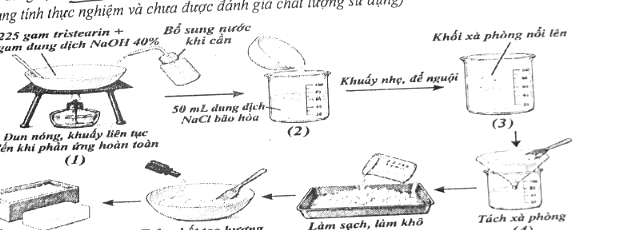
\includegraphics[width=14cm]{images_quangtrung2_hoa12_2102/hinh_p4_cau2_quy_trinh_xa_phong.png}
\end{center}
a) \textit{(0,25 điểm)} Viết phương trình hóa học của phản ứng xà phòng hóa tristearin bằng $\ce{NaOH}$.\\
b) \textit{(0,25 điểm)} Nêu vai trò của dung dịch $\ce{NaCl}$ bão hòa ở giai đoạn (2) trong thí nghiệm.\\
c) \textit{(0,5 điểm)} Một cơ sở sản xuất nhận đơn hàng gồm 48 bánh xà phòng, mỗi bánh có khối lượng $80\text{ gam}$, trong đó sodium stearate chiếm $76{,}5\%$ khối lượng, phần còn lại là các chất phụ gia. Cơ sở sử dụng tristearin nguyên chất phản ứng hoàn toàn với $\ce{NaOH}$ dư. Do hao hụt trong quá trình tách và xử lí sản phẩm, khối lượng sodium stearate thực tế thu được bằng $80\%$ khối lượng tính theo lí thuyết. Tính khối lượng tristearin tối thiểu cần dùng để hoàn thành đơn hàng, theo đơn vị kg.


\loigiai{
a) \textbf{Phương trình hóa học xà phòng hóa tristearin:}
\[ \ce{(C17H35COO)3C3H5 + 3NaOH ->[t^\circ] 3C17H35COONa + C3H5(OH)3} \]
b) \textbf{Vai trò của dung dịch $\ce{NaCl}$ bão hòa ở giai đoạn (2):}\\
Dung dịch $\ce{NaCl}$ bão hòa làm tăng tỉ trọng của dung dịch và làm giảm độ tan của muối sodium stearate (xà phòng), giúp cho xà phòng kết tinh lại và nổi lên trên bề mặt, từ đó dễ dàng tách lọc thu hồi xà phòng.\\
c) \textbf{Tính khối lượng tristearin tối thiểu:}
\begin{itemize}[leftmargin=*,itemsep=1pt]
\item Khối lượng 48 bánh xà phòng: $m_{\text{xà phòng}} = 48 \times 80 = 3840\text{ gam} = 3{,}84\text{ kg}$.
\item Khối lượng sodium stearate thực tế cần có:
\[ m_{\text{TT (stearate)}} = 3840 \times 76{,}5\% = 2937{,}6\text{ gam}. \]
\item Do hiệu suất tách và thu hồi đạt $H = 80\%$, khối lượng sodium stearate lí thuyết cần tạo ra là:
\[ m_{\text{LT (stearate)}} = \dfrac{2937{,}6}{80\%} = 3672\text{ gam}. \]
\item Phân tử khối: $M(\ce{C17H35COONa}) = 306\text{ g/mol}$; $M(\text{tristearin}) = 890\text{ g/mol}$.
\item Số mol sodium stearate lí thuyết: $n_{\text{LT}} = \dfrac{3672}{306} = 12\text{ mol}$.
\item Theo PTHH: $n_{\text{tristearin}} = \dfrac{1}{3} n_{\text{LT}} = \dfrac{12}{3} = 4\text{ mol}$.
\item Khối lượng tristearin tối thiểu cần dùng:
\[ m_{\text{tristearin}} = 4 \times 890 = 3560\text{ gam} = \mathbf{3{,}56\text{ kg}}. \]
\end{itemize}
\textbf{Đáp số: 3,56 kg.}
}

\end{ex}

\vspace{8pt}
\begin{center}
\textbf{---------- HẾT ----------}
\end{center}

\end{document}
